\chapter{Desenvolvemento dos sprints}

A implementación deste proxecto consta de tres ciclos de sprint nos que se desenvolven as dúas compoñentes nas que está dividido. Cada un dos sprints consta das fase de análise, deseño, implementación e probas. Dado que a análise se describiu por completo no capítulo 2, neste capítulo detallaranse o deseño, implementación e probas realizadas para validar os requisitos planificados en cada un dos sprints.

A previsión inicial do contido de cada sprint está recollida no cadro \ref{tab:previsionSprints}, no capítulo de Xestión do proxecto. Neste apartado describirase xa a pila de cada sprint en base ós requisitos definidos, é dicir, o resultado da planificación do sprint. Cabe destacar que para a planificación do sprint non so se ten en conta a relevancia asignada a cada requisito, se non tamén o tempo estimado para levalo a cabo e a súa repercusión no cumprimento dos requisitos non funcionais.

\section{Sprint 1}
Os requisitos funcionais que se inclúen na pila do primeiro sprint son:
\begin{itemize}
\item \ref{req:RF.01}.- Conectar con servidor SOS
\item \ref{req:RF.02}.- Gardar lista de servidores SOS
\item \ref{req:RF.04}.- Xerar capa vectorial cas observacións do servidor
\end{itemize}

Neste ciclo de desenvolvemento levouse a cabo o deseño inicial da interface gráfica para a ventá de conexión co servidor SOS, seguindo como guía as ventás dispoñibles de xeito nativo no QGIS para descargar datos de outros servizos similares (WFS, WMS, WCS), co obxectivo de satisfacer o requisito \ref{req:RNF.03}.

Outra tarefa importante levada a cabo foi a definición dunha estrutura extensible para o módulo de procesamento do XML, de xeito que sexa sinxelo engadir as distintas casuísticas que vaian aparecendo, debido a gran liberdade que dan os estándares SOS e O\&M. Tamén se analizaron distintas posibilidades para o procesamento do XML en Python, sendo todas elas moi similares en canto a funcionalidade, optouse por empregar o módulo para XML das propias librerías Qt para non engadir dependencias innecesarias.

No diagrama \ref{fig:diaClassSOSClient} represéntanse o deseño de clases realizado, que se corresponde coa compoñente SOSClient. Móstranse so os atributos e métodos máis relevantes para entender a función de cada clase, que se representan separadas entre vista e modelo. Agrupadas sobre fondo escuro represéntanse as clases encargadas do procesamento dos documentos XML proporcionados polo servizo SOS.

\begin{sidewaysfigure}
 \centering
 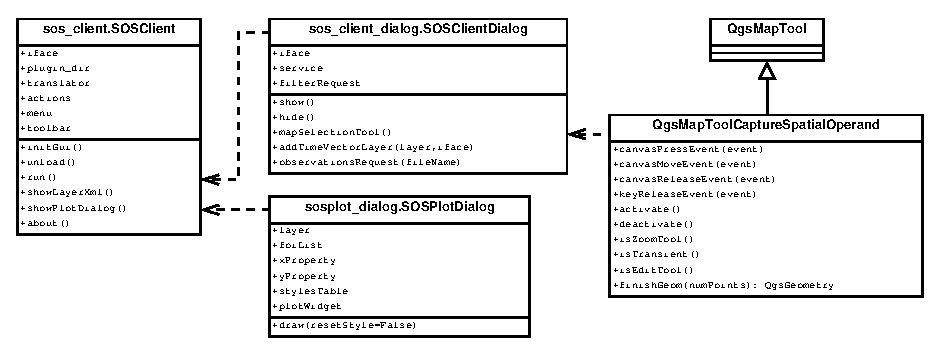
\includegraphics[width=\textwidth]{images/clases_sos_client.eps}
 \caption{Diagrama de clases da compoñente SOS Client}
 \label{fig:diaClassSOSClient}
\end{sidewaysfigure}

As clases máis relevantes da figura \ref{fig:diaClassSOSClient} son:
\begin{description}
\item[WidgetFactory:] É unha factoría de clases que crea, a partir dos XML de definición da interface, as clases cos compoñentes gráficos. A implementación real da vista farase en clases que herdarán da clase correspondente creada por esta factoría.
\item[SOSClientDialog:] É o formulario xeral de comunicación cos servidores SOS. Contén a lóxica de funcionamento da vista e as chamadas necesarias ás clases que forman o modelo.
\item[SensorObservationService:] Esta clase representa o servizo SOS. Créase a partir do XML que define as capacidades do servizo e almacena toda a información necesaria para que a vista poda presentar o usuario as opcións correspondentes para xerar as consultas.
\item[ObservationsLayer:] Esta clase é a encargada de construír a capa vectorial para o QGIS, a partir da clase SOSProvider.
\item[SOSProvider:] Simula unha clase QgsVectorDataProvider\footnote{\url{http://qgis.org/api/classQgsVectorDataProvider.html}}. É pois a clase que fai de intermediaria entre a estrutura de datos real da información da capa e a estrutura manexada polo QGIS.
\item[XMLParserFactory:] É unha factoría para crear as distintas clases para o procesamento dos XML. A partir da etiqueta XML atopada devolve a clase encargada de procesar o nodo.
\item[XMLParser:] Clase base para todas as clases de procesamento de XML.
\end{description}

Tamén se preparou durante este sprint o entorno para a automatización das probas unitarias a través da ferramenta \emph{PyUnit}\footnote{\url{https://docs.python.org/2/library/unittest.html}} e programáronse varios casos de probas para o módulo de procesamento de XML en base a ficheiros de exemplo.

Co obxectivo de validar o incremento xerado leváronse a cabo as seguintes probas:

\testtable{PR.01}{Conexión con servidor SOS}
		  {\begin{itemize}\item \ref{req:RF.01} \item \ref{req:RNF.03}\end{itemize}} %Requerimentos
		  {Compróbase, a parte das probas unitarias automáticas, a conexión con varios servidores SOS.} %Descripción
		  {\begin{itemize}
		  \item A información das capacidades do servizo visualízanse en formato HTML cos estilos propios de QGIS.
		  \item As ofertas dispoñibles visualízanse nunha caixa de selección, e as propiedades e procedementos relacionados en sendas listas nas que se poden marcar e desmarcar. Estas listas actualízanse correctamente ó modificar a oferta seleccionada.
		  \end{itemize}} %Resultado
		  
\testtable{PR.02}{Xestión de servidores}
		  {\begin{itemize}\item \ref{req:RF.02} \item \ref{req:RNF.03}\end{itemize}} %Requerimentos
		  {Próbanse as funcionalidades de alta, baixa e modificación de conexións na interface gráfica, así coma o correcto gardado entre distintas execucións da aplicación QGIS.} %Descripción
		  {Todas as operacións funcionan correctamente.} %Resultado

\testtable{PR.03}{Descargar observacións}
		  {\begin{itemize}\item \ref{req:RF.04} \\\end{itemize}} %Requerimentos
		  {Compróbase a execución da operación \emph{GetObservations} contra varios servidores.} %Descripción
		  {\begin{itemize}
		  \item O XML descárgase correctamente.
		  \item O XML procesase e obtéñense as xeometrías contidas no mesmo coas que se crea unha capa vectorial en memoria no QGIS.
		  \end{itemize}} %Resultado
		  
O \ref{req:RF.04} cubriuse parcialmente, pois aínda que se podían visualizar no mapa os puntos correspondentes as observacións o resto de información do XML se trata correctamente.

Tendo en conta a matriz de trazabilidade do cadro \ref{tab:trazaRequisitos}, este primeiro incremento non resolve ningún caso de uso completo.

\section{Sprint 2}
Na pila do segundo sprint inclúense os seguintes requisitos funcionais:
\begin{itemize}
\item \ref{req:RF.04}.- Xerar capa vectorial cas observacións do servidor (continuación)
\item \ref{req:RF.03}.- Visualizar XML das capacidades do servidor
\item \ref{req:RF.05}.- Permitir filtrado básico das observacións a descargar
\item \ref{req:RF.07}.- Xerar petición de observacións manualmente
\item \ref{req:RF.11}.- Xerar animación no visor de mapas
\item \ref{req:RF.08}.- Xerar gráfica propiedade vs tempo
\end{itemize}

No segundo ciclo de sprint conclúese o módulo de procesamento XML para interpretar correctamente todos os datos das observacións resultado da operación \emph{GetObservations}, tanto co modelo \emph{Observations} como co \emph{Measurements}. Amais comprobase que requisitos debe cumprir a capa para poder ser xestionada a través do plugin \emph{TimeManager}, e impleméntase o proceso de creación da capa tendo en conta estes requisitos.

Tamén se implementan os filtros básicos de observacións, e por ser de utilidade para o proceso de desenvolvemento e probas tamén se implementa a visualización do XML das capacidades do servidor e a posibilidade de visualizar e editar o XML xerado para a petición de observacións.

En canto a xeración de gráficas realízanse varias probas coa librería matplotlib.

Co obxectivo de validar o incremento xerado leváronse a cabo as seguintes probas:

\testtable{PR.04}{Procesamento de XML con observacións en formato \emph{Observations} e \emph{Measurements}}
		  {\begin{itemize}\item \ref{req:RF.04} \\\end{itemize}} %Requerimentos
		  {Codifícanse probas unitarias para a validación do módulo de procesamento so XML de observacións nos dous formatos, en base a ficheiros de exemplos dos servidores SOS do CiTIUS.} %Descripción
		  {\begin{itemize}
		  \item O XML procesase correctamente, detectando os campos de tipo tempo, os numéricos e as cadeas de texto.
		  \item A partir da estrutura de datos xerada a partir do XML crease correctamente unha capa vectorial no QGIS, con todos os campos contidos na observación e cos valores correctos.
		  \end{itemize}} %Resultado

\testtable{PR.05}{Xeración de filtros para \emph{GetObservations}}
		  {\begin{itemize}\item \ref{req:RF.03} \item \ref{req:RF.05} \item \ref{req:RF.07}\end{itemize}} %Requerimentos
		  {Comprobar que os obxectos de interface conteñen os valores correctos segundo as capacidades do SOS e que o XML que se xera a través das distintas opcións de interface é válido.} %Descripción
		  {\begin{itemize}
		  \item Comprobase conectando con varios servidores que as opcións habilitadas nas distintas lapelas de filtros se corresponden coas capacidades definidas no XML.
		  \item A lista de sensores seleccionados e a de entidades de interese, así como o operador e operandos dos filtros de tempo inclúense correctamente no XML para a petición \emph{GetObservations}.
		  \end{itemize}} %Resultado

\testtable{PR.06}{Xestionar capa co \emph{TimeManager}}
		  {\begin{itemize}\item \ref{req:RF.04} \item \ref{req:RF.11} \end{itemize}} %Requerimentos
		  {Comprobar o correcto funcionamento do plugin \emph{TimeManager} coa capa creada.} %Descripción
		  {\begin{itemize}
		  \item Comprobase que a capa se engade á lista das xestionadas polo \emph{TimeManager} de xeito satisfactorio.
		  \item Verificase que o campo de tempo se interpreta correctamente.
		  \item Comprobase o funcionamento xeral do \emph{TimeManager} con varias capas de observacións.
		  \end{itemize}} %Resultado
		  
\testtable{PR.07}{Gráfica tempo \emph{vs} propiedade}
		  {\begin{itemize}\item \ref{req:RF.08} \\\end{itemize}} %Requerimentos
		  {Xerar gráfica co tempo no eixo X e a propiedade no Y.} %Descripción
		  {\begin{itemize}
		  \item A gráfica contén todas as observacións co mesmo \emph{foi} que a entidade seleccionada no mapa.
		  \item As observacións ordénanse polo campo tempo de xeito que se poda trazar unha liña que as una.
		  \item Ós valores do eixo X dáselles formato de tempo.
		  \end{itemize}} %Resultado
		  
Tendo en conta a matriz de trazabilidade do cadro \ref{tab:trazaRequisitos}, con este segundo incremento cúbrense os casos de uso \ref{uc:CU.01} e \ref{uc:CU.04}.
		  
\section{Sprint 3}
Na pila do terceiro sprint inclúense os seguintes requisitos funcionais:
\begin{itemize}
\item \ref{req:RF.06}.- Permitir filtrado avanzado das observacións a descargar
\item \ref{req:RF.09}.- Xerar gráfica para enfrontar dúas propiedades
\item \ref{req:RF.10}.- Xerar gráfica con varias series
\end{itemize}

Neste incremento habilítase a ferramenta para introducir o filtro espacial seleccionando a xeometría directamente sobre o mapa, segundo o tipo de operando seleccionado.

Tamén se modifica a visualización de gráficas para permitir seleccionar as propiedades a visualizar, traballar con varias \emph{foi} seleccionadas e permitir modificar os estilos e textos da gráfica. Esta tarefa implica o deseño tanto da interface gráfica como da estrutura de clases da compoñente SOSPlot, que se representa no diagrama \ref{fig:diaClassSOSPlot}. Móstranse agrupadas todas as clases que cumpren co rol de \emph{Delegate}. As demais correspóndense coa vista, pois o modelo da compoñente SOSPlot está soportado por clases internas do QGIS (QgsVectorLayer) e de matplotlib (Line2D).

\begin{figure}
 \centering
 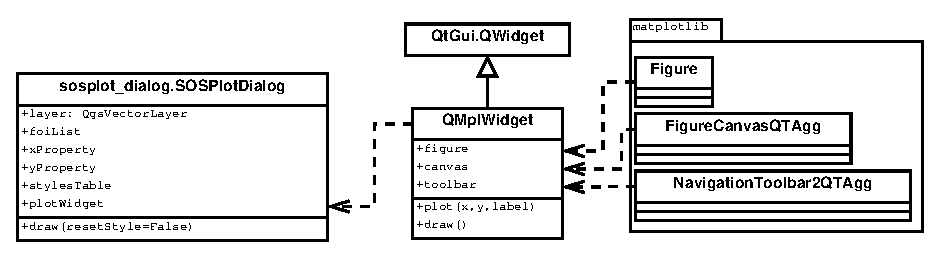
\includegraphics[width=\textwidth]{images/clases_sos_plot.eps}
 \caption{Diagrama de clases da compoñente SOS Plot}
 \label{fig:diaClassSOSPlot}
\end{figure}

As clases máis relevantes da figura \ref{fig:diaClassSOSPlot} son:
\begin{description}
\item[WidgetFactory:] Factoría para a xeración das compoñentes gráficas.
\item[SOSPlotDialog:] É o formulario de visualización de gráficos. Filtra e transforma os datos da capa vectorial activa para visualizalos no QMplWidget e conecta os distintos \emph{Delegates} co modelo.
\item[QMplWidget:] Clase que amalgama os obxectos da librería matplotlib para a visualización de gráficos.
\end{description}
\newpage
Co obxectivo de validar o incremento xerado leváronse a cabo as seguintes probas:

\testtable{PR.08}{Filtros espaciais}
		  {\begin{itemize}\item \ref{req:RF.06} \\\end{itemize}} %Requerimentos
		  {Comprobar o correcto funcionamento da ferramenta de selección de xeometrías e a inclusión no XML do filtro correspondente.} %Descripción
		  {\begin{itemize}
		  \item A ferramenta de selección permite debuxar rectángulos (indicando dous puntos), polígonos, liñas e puntos.
		  \item A xeometría debuxada no mapa transformase correctamente ó formato GML e inclúese no XML para a petición \emph{GetObservations}.
		  \end{itemize}} %Resultado
		  
\testtable{PR.09}{Xeración de gráficas con varias series}
		  {\begin{itemize}\item \ref{req:RF.10} \\\end{itemize}} %Requerimentos
		  {Compróbanse a xeración de gráficas a partir de varias entidades seleccionadas, de forma que cada \emph{foi} teña un estilo distinto.} %Descripción
		  {\begin{itemize}
		  \item Permítese xerar a gráfica con varias entidades seleccionadas. Para cada \emph{foi} distinto ordénanse os datos e debúxase a liña con unha cor distinta.
		  \item Permítese modificar a cor e estilo de cada liña e dos marcadores.
		  \end{itemize}} %Resultado
		  
\testtable{PR.10}{Personalización das propiedades das gráficas}
		  {\begin{itemize}\item \ref{req:RF.09} \\\end{itemize}} %Requerimentos
		  {Verificar que se poden modificar as distintas propiedades da gráfica, incluídas a propiedade a representar en cada eixo.} %Descripción
		  {\begin{itemize}
		  \item Pódense seleccionar o campo da capa a usar no eixo X e no eixo Y, así como por cal dos dous ordenar os datos para trazar liñas.
		  \item Permítese modificar os límites dos eixos X e Y manualmente.
		  \item Pódense modificar outras propiedades da gráfica como o título, as etiquetas e o formato de tempo.
		  \end{itemize}} %Resultado
		  
Tendo en conta a matriz de trazabilidade do cadro \ref{tab:trazaRequisitos}, con este terceiro incremento a aplicación permite levar a cabo os catro casos de uso definidos.